%% AMS-LaTeX Created with the Wolfram Language : www.wolfram.com

\documentclass{article}
\usepackage{amsmath, amssymb, graphics, setspace}

\newcommand{\mathsym}[1]{{}}
\newcommand{\unicode}[1]{{}}

\newcounter{mathematicadefinition}
\newcounter{mathematicaproposition}
\newcounter{mathematicafigurecaption}
\begin{document}

\title{Design of NEO ID}
\author{Draft Version}
\date{}
\maketitle


\section{Introduction}


\subsection{Background}



Each time we carry out vital communication in any distributed computer system such as the Internet, we face an inherent risk. This risk arises because
we can never be completely certain about the trustworthiness of entities that mediate our online interactions. (* REF NEEDED *) (* EXAMPLE NEEDED:
CHATING ONLINE, HTTPS AND OTHER SCENARIOS*)



To minimise this risk, users must be given the chance to check the ID with each other on the network. (* DETAILS NEEDED *)



Well known techniques to ensure that something is authenticated have been developed and strengthened, and these techniques include cryptographic
algorithms for secrecy and digital signatures, authentication protocols for proving authenticity, and access control methods for managing authorisation.
(* REF NEEDED *) However, these techniques do not say much about the wider notion of an entity{'}s ID. For example, cryptographic algorithms cannot
say if a piece of digitally signed code has been authored by competent programmers and a signed public-key certificate does not tell you if the owner
is an industrial spy. (* REF NEEDED *)



Acting on behalf of a human being, any online identity is an extension of a person, and therefore must be given the same capability as humans to
manage and reason about trust. In the following of this paper, we will explain why traditional network security mechanisms and ID management solutions
are incomplete, and provide a general ID management protocol.


\subsection{Related Work}



(* TODO *)



(* ONT ID *)



(* PKI $\&$ CertLedger *)



(* Comparisons between these solutions *)


\section{Definition}



(* TODO *)



(* We have a definition before (version 2019-03-18), but it may need to be refined. *)


\section{Solution}



(* TODO *)


\subsection{Overview}



We here propose a distributed ID framework that satisfies the following properties: (* REF NEEDED *) (* REFINE NEEDED *)

evolves trust based on a graph of trust network, whose trust metric is expressive, yet tractable;

protects user anonymity, whilst being resistant to {``}Sybil attacks{''} (and enhancing detection of two collusion attacks);

integrates a risk-aware decision module;



Our solution consists of the following three parts:

Trust Model



The trust model describes the rules of trust in a distributed network.



(* still not sure for whether the trust model should be memoryless *)

Game Model



The game model describes the benefits and penalties of trust and guarantee.

Privacy Model



The privacy model describes the privacy protection scheme for users{'} online data.


\subsection{Trust Model}



(* TODO *)


\subsubsection{Introduction}



Trust is a common phenomenon. Indeed, it has been argued that we as humans would not even be able to face the complexities of the world without resorting
to trust, because it is with trust that we are able to reason sensibly about the possibilities of everyday life.



What is trust? Trust is a subjective assessment of another's influence in terms of the extent of one's perception about the quality and significance
of another's impact over one's outcomes in a given situation, such that one's expectation of, openness to, and inclination toward such influence
provide a sense of control over the potential outcomes of the situation. Several definitions of the human notion of trust have been proposed during
the last years in different domains from sociology, psychology to political and business science. These definitions may even change in accordance
with the application domain.



Let us first define trust with a commonly accepted definition: (* REF NEEDED *)



Trust (or, symmetrically, distrust) is a particular level of the subjective probability with which an agent will perform a particular action, both
before [we] can monitor such action (or independently of his capacity of ever to be able to monitor it) and in a context in which it affects [our]
own action.



From this definition, three properties of trust emerge: subjectiveness, context-dependence, and dynamism. The same behavior may lead to different
trust levels in different trusting entities, hence subjectiveness qualifies trust. As trust (e.g., in giving good advices) in one context (e.g.,
academia) does not necessarily transfer to another context (e.g., industry), we add context-dependence to the list of trust properties. Finally,
the fact that trust increases after successful observations, while it decays over time exemplifies its dynamism. As a result, trust evolution must
embed the notion of time.



(* REPUTATION $\&$ TRUST *)



Centralised protocols are protocols which use a well-known common trusted intermediary, call it the trusted authority, to form a trust relationship
between two mutually distrusting entities. (* LIKE CA *) This need to refer to a centrally trusted point poses a major problem as a general trust
framework, because the assumed objectivity of trust will not work. In our definition of trust, trust is subjective. Furthermore, a TA can never be
a good enough recommender for everyone in a large distributed system. Its credibility depletes, and its recommendations increase in uncertainty,
as its community of trustees grows. A decentralised approach to trust management makes sense, simply because trust decisions cannot be forced onto
entities. (* REF NEEDED *)



If a secure system is desired, trust assumptions must be explicit. It is insufficient to say that Alice trusts Bob. More qualification is required:
What does Alice trust Bob for, how much does Alice trust Bob and under what circumstances does that trust relationship hold or break? (* REF NEEDED
*)



(* BEGIN Transitivity of trust $\&$ REF NEEDED *)\\
Most authentication protocols rely on the basic assumption that trust is transitive, i.e. if Alice trusts Bob, and Bob trusts Cathy, then it follows
that Alice trusts Cathy. This, however, is an erroneous assumption. Trust is not transitive. If Alice trusts Bob, and Bob trusts Cathy, it does not
follow that Alice trusts Cathy. Alice's trust in Bob has no relation whatsoever to Bob's trust in Cathy. The decision on whether to trust or distrust
a subject, or a given authentication chain is ultimately made by the entity, and cannot be automated by any protocol\\
(* END Transitivity of trust *)



(* FOLLOWING DESCRIPTIONS NEED TO BE REFINED *)



The taking of risk is necessary in ongoing relationships, both in order to confirm the trust that already exists, and to strengthen it, should the
risk be justified. On the other hand, if the risk is not justified and the other party defects, trust is revised downwards dramatically. Trust is
often founded on evidence, but even when our expectations are well grounded there is an element of risk in trust, a chance that those whom we trust
will not act as expected.



(* TODO *)



Our trust model is memoryless. We treat the trust model as a time-independent state.



Distributed trust frameworks may support trust and thus foster collaboration in an hostile pervasive computing environment. To design a general distributed
trust framework, one needs to identify its desirable properties. Our framework:


\item is distributed;


\item protects user anonymity, whilst providing accountability; (* with privacy model *)


\item is lightweight in terms of both required storage and scalability;


\item minimizes bandwidth demand;


\item is robust to common attacks;


\item evolves (social) trust as humans do (e.g., trust evolves based on reputation information); (* not sure *)


\item supports both types of recommendations (good and bad ones);


\item incorporates the three classical dimensions of computational trust: context, subjectiveness, and time;


\item is integrated with a decision module;


\item has a trust metric that is expressive, yet tractable;


\subsubsection{Definition}


\subsubsubsection{Trust Value}



There are many ways to quantify trust, but to simplify the problem, we choose to represent trust as a continuous variable over a specific range \([-1,
+1]\).

\(\text{Definition} \arabic{mathematicadefinition}.\)Trust value \(a\) is a scalar to describe how much one trusts another. Trust here refers to
direct trust.



Here are some properties of trust value \(a\):

\(\text{Proposition} \arabic{mathematicaproposition}.\)
\item The maximum value of 
\item \(a\)
\item  is 
\item \(+1\)
\item  which means blind trust

\(\text{Proposition} \arabic{mathematicaproposition}.\)
\item The minium value of 
\item \(a\)
\item  is 
\item \(-1\)
\item  which means complete distrust

\(\text{Proposition} \arabic{mathematicaproposition}.\)
\item The trust value \(0\)
\item  is a neutral value which means no trust nor distrust.

\(\text{Proposition} \arabic{mathematicaproposition}.\)
\item The greater the \(a\)
\item , the more trust




\item Thus we know the domain of \(a\)

\(a\in \mathbf{a}=[-1,+1]\)



Here is a possible stratification of trust values:


\caption{Table 1. Possible stratification of trust values} 


\begin{tabular}
\(\begin{array}{lc}
\hline
 \text{Value Range} & \text{Lable} \\
\hline
 +1 & \text{Blind Trust} \\
\hline
 \text{[0.9, 1)} & \text{Very High Trust} \\
 \text{[0.75, 0.9)} & \text{High Trust} \\
 \text{[0.5, 0.75)} & \text{High Medium Trust} \\
 \text{[0.25, 0.5)} & \text{Low Medium Trust} \\
 \text{(0, 0.25)} & \text{Low Trust} \\
 0 & \text{No Trust or Distrust} \\
 \text{(-0.25, 0)} & \text{Low Distrust} \\
 \text{(-0.5, -0.25]} & \text{Low Medium Distrust} \\
 \text{(-0.75, -0.5]} & \text{High Medium Distrust} \\
 \text{(-0.9, -0.75]} & \text{High Distrust} \\
 \text{(-1, -0.9]} & \text{Very High Distrust} \\
 -1 & \text{Complete Distrust} \\
\end{array}\)
\end{tabular}


\subsubsubsection{Trust Network}

\(\text{Definition} \arabic{mathematicadefinition}.\)A trust network is a weighted directed graph \(\mathcal{G}=(\mathcal{V},\mathcal{E},A)\):\(\mathcal{V}\)
is the set of vertices of the graph. Each vertex represents an entity (people, organization, group, assets, proposition); \(\mathcal{E}\) is the
set of edges of the graph. Each edge from vertex \(i\) to vertex \(j\) means that there is a direct trust (or distrust) from \(i\) to \(j\); \(A\)
is the weight adjacency matrix of the graph where \(a_{i,j}\) denotes the scalar entry in the \((i,j)\)-th position which means the trust value from
\(i\) to \(j\).



Here are some properties of trust network \(\mathcal{G}=(\mathcal{V},\mathcal{E},A)\) which we can inference from above:

\(\text{Proposition} \arabic{mathematicaproposition}.\)All the trust values in the weight adjacency matrix \(A\) are in the domain of \([-1,+1]\)

\(a_{i,j}\in [-1,+1] \text{for} \forall i,j\in \mathcal{V}\)

\(\text{Proposition} \arabic{mathematicaproposition}.\)if \(i\) remains neutral about \(j\), the trust value is \(0\).

\(a_{i,j}=0 \text{if} (i,j)\notin \mathcal{E}\)


\subsubsubsection{Trust Process Function}

\(\text{Definition} \arabic{mathematicadefinition}.\)Trust process function is a function \(f_{\mathcal{G}}:(\mathcal{V},\mathcal{V})\to \mathbf{a}\)
on the trust network. We can use \(f_{\mathcal{G}}(x,y)\) to solve a overall trust metric from the trustor \(x\) to the trustee \(y\).



We have some assumptions about the trust process function \(f\):

\(\text{Proposition} \arabic{mathematicaproposition}.\)Any increment of trust value in the trust network will never decrease the overall trust from
one to another.

\(\frac{\partial f}{\partial a_{i,j}}\geqslant 0 \text{for} \forall i,j\in \mathcal{V}\)

\(\text{Proposition} \arabic{mathematicaproposition}.\)Trust will gradually decay during the process of transition.



For example, we have \(f_{\mathcal{G}_1}(x,y)\) to describe the overall trust from \(x\) to \(y\) in figure 1, if we add a trust relation from \(y\)
to \(v\), the graph will be figure 2. We know \(x\) may have more confidence to \(y\) than \(v\) because the trust value from \(x\) to \(v\) rely
on the trust from \(x\) to \(y\).

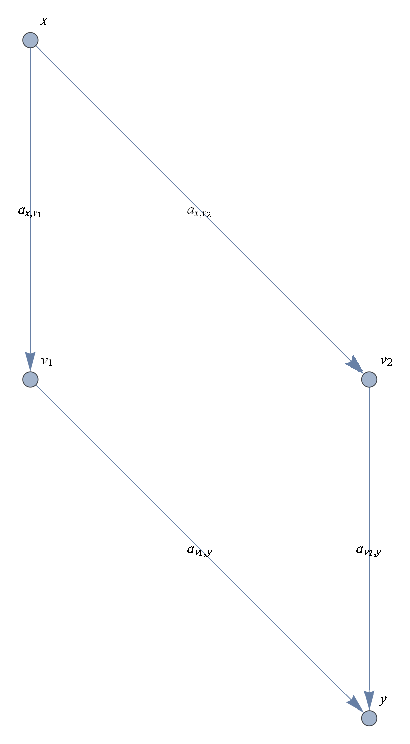
\includegraphics{NEOID_gr1.eps}


\caption{\(\text{Figure} \arabic{mathematicafigurecaption}.\)The trust network before adding \(v\)}


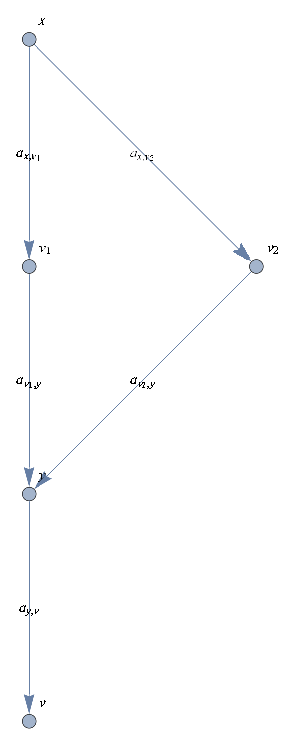
\includegraphics{NEOID_gr2.eps}


\caption{\(\text{Figure} \arabic{mathematicafigurecaption}.\)The trust network after adding \(v\)}




Thus we assume the following expression

\(\frac{f_{\mathcal{G}^{\oplus }}(x,v)}{f_{\mathcal{G}}(x,y)}\in [-1,+1]\)

\(\frac{f_{\mathcal{G}^{\ominus }}(v,y)}{f_{\mathcal{G}}(x,y)}\in [-1,+1]\)

\(\mathcal{G}^{\oplus }=\left(\mathcal{V}\cup \{v\},\mathcal{E}\cup \{(y,v)\},\left(
\begin{array}{cc}
 A & \left(
\begin{array}{c}
 0 \\
 \vdots \\
a_{y,v} \\
 \vdots \\
0 \\
\end{array}
\right) \\
 \square  & a_{v,v} \\
\end{array}
\right)\right)\)

\(\mathcal{G}^{\ominus }=\left(\mathcal{V}\cup \{v\},\mathcal{E}\cup \{(v,x)\},\left(
\begin{array}{cc}
 A & \square  \\
 \left(
\begin{array}{ccccc}
 0 & \cdots  & a_{v,x} & \cdots  & 0 \\
\end{array}
\right) & a_{v,v} \\
\end{array}
\right)\right)\)

\(\text{Proposition} \arabic{mathematicaproposition}.\)More positive recommends are better.



For example, we have \(f_{\mathcal{G}_3}(x,y)\) to describe the overall trust from \(x\) to \(y\) in figure 3, we have only one proof-chain to describe
the trust from \(x\) to \(y\). If there are more proof chains like \(x\to v\to y\) in figure 4, it would be useful.


\includegraphics{NEOID_gr3.eps}


\caption{\(\text{Figure} \arabic{mathematicafigurecaption}.\)The trust network before adding \(v\)}



\includegraphics{NEOID_gr4.eps}


\caption{\(\text{Figure} \arabic{mathematicafigurecaption}.\)The trust network after adding \(v\)}




Thus we assume the following expression:

\(f_{\mathcal{G}^{\otimes }}(x,y)-f_{\mathcal{G}}(x,y)\left\{
\begin{array}{cc}
 \geq 0 & f_{\mathcal{G}^{\odot }}(x,y)\geq  0 \\
 \leq 0 & f_{\mathcal{G}^{\odot }}(x,y)\leq \text{  }0 \\
\end{array}
\right.\)

\(\mathcal{G}^{\otimes }=\left(\mathcal{V}\cup \{v\},\mathcal{E}\cup \{(x,v),(v,y)\},\left(
\begin{array}{cc}
 A & \left(
\begin{array}{c}
 0 \\
 \vdots \\
a_{x,v} \\
 \vdots \\
0 \\
\end{array}
\right) \\
 \left(
\begin{array}{ccccc}
 0 & \cdots  & a_{v,y} & \cdots  & 0 \\
\end{array}
\right) & a_{v,v} \\
\end{array}
\right)\right)\)

\(\mathcal{G}^{\odot }=\left(\{x,v,y\},\{(x,v),(v,y)\},\left(
\begin{array}{ccc}
 a_{x,x} & a_{x,v} & \square  \\
 \square  & a_{v,v} & a_{v,y} \\
 \square  & \square  & a_{y,y} \\
\end{array}
\right)\right)\)



(* TO BE REMOVED BEGIN *)


\item \(a_{x,y}^{(1)}=a_{x,y}\)


\item \(a_{x,y}^{(n)}=\underset{k}{\oplus }\left(a_{x,k}^{(n-1)}\otimes a_{k,y}\right)\)


\item \(f_{\mathcal{G}}(x,y)=a_{x,y}^{(n)}\)


\item \(\underset{k}{\oplus }\left(x_k\right)\geqslant \max _k\left(x_k\right)\)


\item \(x\otimes y\leqslant \min _k\left(x_k\right)\)


\item \(\frac{\partial \oplus }{\partial x}\geqslant 0\)


\item \(\frac{\partial \otimes }{\partial x}\geqslant 0\)



(* Additional Assumption may be used *)



(* DESCRIPTION NEEDED *)


\item \(\oplus (x,y)=\oplus (y,x)\)


\item \(x\otimes y=y\otimes x\)


\item \((x\otimes y)\otimes z=x\otimes (y\otimes z)\)


\item \(\oplus (x,y)\otimes z=\oplus (x\otimes z,y\otimes z)\)



(* TO BE REMOVED END *)



(* OLD TEXT BEGIN *)


\subsubsection{Solution}


\subsubsubsection{Normal Reliable Direct Trust}



(* DESCRIPTION NEEDED *)

\(f_{\mathcal{G}}(x,y)=\begin{cases}
 1 & a_{x,y}=1 \\
 0 & \text{else}
\end{cases}\)


\subsubsubsection{Normal Unreliable Direct Trust}



(* DESCRIPTION NEEDED *)

\(f_{\mathcal{G}}(x,y)=\begin{cases}
 a_{x,y} & a_{x,y}>0 \\
 0 & \text{else}
\end{cases}\)


\subsubsubsection{Normal Reliable Recommended Trust}



(* DESCRIPTION NEEDED *)

\(f_{\mathcal{G}}(x,y)=\begin{cases}
 1 & \exists \pmb{p}\in \text{Permutation}(\mathcal{V}),\pmb{p}_i=x,\pmb{p}_j=y,i<j,\text{for} \forall k\in [i,j-1] a_{\pmb{p}_k,\pmb{p}_{k+1}}=1
\\
 0 & \text{else}
\end{cases}\)


\subsubsubsection{Normal Unreliable Recommended Trust}



(* DESCRIPTION NEEDED *)



(* Simple Recommended Trust *)

\(f_{\mathcal{G}}(x,y)=e^{\frac{1}{\sum _i^{\mathcal{V}} \frac{1}{\text{Log}\left[\max \left(a_{i,y},0\right) \max \left(a_{x,i},0\right)\right]}}}\)



(* Maximum Trust Path *)

\(f_{\mathcal{G}}(x,y)=\max \left\{\left.\prod _{k=i}^{j-1} \max \left(a_{\pmb{p}_k,\pmb{p}_{k+1}},0\right)\right|\pmb{p}\in \text{Permutation}(\mathcal{V}),\pmb{p}_i=x,\pmb{p}_j=y,i<j\right\}\)



(* TODO *)



(* MARKOV METHOD *)



(* BAYESIAN METHOD - PREFERED *)



(* RESISTANCE DISTANCE METHOD - FOR Symmetrical *)



(* REFER https://www.nr.no/$\sim $abie/Papers/TR133.pdf *)


\subsubsubsection{Extended Reliable Direct Trust}



(* DESCRIPTION NEEDED *)

\(f_{\mathcal{G}}(x,y)=\begin{cases}
 a_{x,y} & a_{x,y}^2=1 \\
 0 & \text{else}
\end{cases}\)


\subsubsubsection{Extended Unreliable Direct Trust}



(* DESCRIPTION NEEDED *)

\(f_{\mathcal{G}}(x,y)=a_{x,y}\)


\subsubsubsection{Extended Reliable Recommended Trust}



(* DESCRIPTION NEEDED *)



(* PASSIVE VERSION *)

\(f_{\mathcal{G}}(x,y)=\begin{cases}
 \Pi  & \exists \pmb{p}\in \text{Permutation}(\mathcal{V}),\pmb{p}_i=x,\pmb{p}_j=y,i<j,\Pi =\prod _{k=i}^{j-1} a_{\pmb{p}_k,\pmb{p}_{k+1}},\Pi ^2=1
\\
 0 & \text{else}
\end{cases}\)



(* INITIATIVE VERISON *)





\(f_{\mathcal{G}}(x,y)=\begin{cases}
 
\begin{array}{ll}
 1 & \forall \pmb{p}\in \left\{\pmb{p}|\pmb{p}\in \text{Permutation}(\mathcal{V}),p_i=x,\pmb{p}_j=y,i<j,\Pi =\prod _{k=i}^{j-1} a_{\pmb{p}_k,\pmb{p}_{k+1}},\Pi
^2=1\right\},\Pi =1 \\
 -1 & \forall \pmb{p}\in \left\{\pmb{p}|\pmb{p}\in \text{Permutation}(\mathcal{V}),p_i=x,\pmb{p}_j=y,i<j,\Pi =\prod _{k=i}^{j-1} a_{\pmb{p}_k,\pmb{p}_{k+1}},\Pi
^2=1\right\},\Pi =-1 \\
 0 & \text{else} \\
\end{array}

\end{cases}\)


\subsubsubsection{Extended Unreliable Recommended Trust}



(* DESCRIPTION NEEDED *)



(* TODO *)



(* OLD TEXT END *)


\subsubsection{Protocol}



(* REFINE THE FOLLOWING DEFS to SOME STANDARD FORMAT *)



(* SOME FIELD MAY NEED TO RENAME *)

message GLOBAL$\_$TRUST$\_$NETWORK $\{$\\
\hspace*{2.ex} repeated ENTITY entities = 1;\\
\hspace*{2.ex} repeated AUTHORIZATION authorizations = 2;\\
$\}$\\
\\
message LOCAL$\_$TRUST$\_$PROFILE $\{$\\
\hspace*{2.ex} repeated AUTHORIZATION authorizations = 1;\\
\hspace*{2.ex} optional TRUST$\_$PROCESS$\_$FUNCTION trust$\_$process$\_$function = 2;\\
$\}$\\
\\
message TRUST$\_$PROOF $\{$\\
\hspace*{2.ex} repeated AUTHORIZATION authorizations = 1;\\
$\}$\\
\\
message ENTITY $\{$\\
\hspace*{2.ex} PUBLIC$\_$KEY id = 1;\\
\hspace*{2.ex} ENTITY$\_$TYPE type = 2;\\
\hspace*{2.ex} repeated DOMAIN domains = 3;\\
\hspace*{2.ex} optional META metadata = 4;\\
$\}$\\
\\
message AUTHORIZATION $\{$\\
\hspace*{2.ex} PUBLIC$\_$KEY trustor = 1;\\
\hspace*{2.ex} PUBLIC$\_$KEY trustee = 2;\\
\hspace*{2.ex} TRUST$\_$VALUE trust$\_$value = 3;\\
\hspace*{2.ex} VALID$\_$TIME valid$\_$time = 4;\\
\hspace*{2.ex} optional META metadata = 5;\\
\hspace*{2.ex} SIGNATURE signature = 6;\\
$\}$\\
\\
enum ENTITY$\_$TYPE $\{$\\
\hspace*{2.ex} TRUSTEE = 1;\\
\hspace*{2.ex} TRUSTOR = 2;\\
\hspace*{2.ex} RECOMMENDER = 3;\\
\hspace*{2.ex} GROUP = 4;\\
$\}$


\subsection{Game Model}



(* TODO *)



(* Limited rationality *)


\subsection{Privacy Model}



(* TODO *)


\subsection{Protocol Design}



(* TODO *)


\section{Analysis}



(* TODO *)


\subsection{Generalization}



We can describe the traditional ID solutions (including CID and DID) as some special cases of NEO ID which shows NEO ID is a more generalized solution.



(* TODO *)


\subsection{Performance}



We will show some performance metrics of NEO ID and then we can compare NEO ID with other solutions under these context.



(* TODO *)


\subsection{Experiments}



(* TODO *)


\section{Conclusion}



(* TODO *)

\end{document}
